\documentclass{article}
\usepackage[utf8]{inputenc}
\parskip = 0.75em
\parindent = 10mm
\def\baselinestretch{1}
\usepackage {float}
\usepackage{listings}
\usepackage{subcaption}
\usepackage[usenames]{color}
\usepackage[numbers,sort&compress]{natbib}
\usepackage{multirow, array}
\usepackage[spanish]{babel}
	\deactivatetilden
	\spanishdecimal{.}
	\addto\captionsspanish{\def\tablename{Tabla}}
	\addto\captionsspanish{\def\listtablename{\'Indice de tablas}}

\usepackage{amsmath,amsfonts,amssymb}
	\allowdisplaybreaks[4]
\usepackage{graphicx}
	\graphicspath{{Figuras/}}
\usepackage[clearempty,pagestyles]{titlesec}
\usepackage{anysize}

\def\baselinestretch{1.5}
\papersize{27.9cm}{21.5cm} 
\marginsize{2cm}{2cm}{1cm}{1cm}

\begin{document}


	\begin{center}
	\huge{\textbf{Tarea 4 Simulación de Diagramas de Voronoi}}\\
	
	\textsc{ \Large Susana Ruiz Nuñez}
	\end{center}


\section{Planteamiento del problema} 
Se toma de un espacio bidimensional \cite{satu} una zona con medidas conocidas que contiene $k$ puntos semilla $p_i$, representados por sus coordenadas. Lo que se busca es dividir esa zona en regiones llamadas celdas de Voronoi de tal forma que todos los puntos que pertenecen a la región de $p_i$ estén más cerca de esa semilla que a cualquier otra. Se requiere examinar de manera sistemática el efecto del número de semillas y del tamaño de la zona en la distribución en las grietas que se forman en términos de la mayor distancia euclideana entre la grieta y el exterior de la pieza.


\section{Metodología}
Se parte de un modelo base \cite{satu}, donde se tiene representadas las celdas del diagrama Voronoi, las semillas y su propagación dadas por una probabilidad inicial de 0.9; lo que posteriormente se cambia para fines del estudio. El equipo donde se realiza el proyecto cuenta con AMD Ryzen 3 3200U with Radeon Vega Mobile Gfx  4 CPUs, ~2.6GHz, dos núcleos físicos y dos virtuales.\\
Con el fin de estudiar el comportamiento cuando cambia el tamaño de la zona y el número de semillas por zona, se crean dos listas que tendrán los diferentes valores de las zonas y la inclusión de las semillas, lo que se adjunta al código en forma de for para cada uno de los dos aspectos a estudiar. Las pruebas se realizaron para un total de 50 iteraciones.
  

\begin{lstlisting}[language=Python]
	size = [60, 80, 100, 150]
	tamSemilla = [d for d in np.arange(0.2, 0.8, 0.2)]
	for n in size:
		datos = []
		for t in tamSemilla:
			semillas = []
				k = n * t
				for s in range(k):
\end{lstlisting}

Para calcular las distancias de las grietas que llegaron más lejos simplemente se usó la ya conocida fórmula de distancia euclediana \cite{satu2}.
\begin{lstlisting}[language=Python]
	distEucl = sqrt(((1)**2) + ((1)**2))
\end{lstlisting}

\section{Resultados}
Como se muestra en las gráficas de la figura 1 tiende a haber un comportamiento más estable al aumentar el porciento de aparición de número de semillas y por supuesto de ocurrir grietas disminuye el largo de las mismas. Esto se debe a que al tener un alto número de semillas, aumenta las fronteras por las que puede seguir su camino la grieta y se vuelve una tarea más lenta la del aumento de la grieta.

\begin{figure}
	\centering
	\begin{subfigure}[b]{0.45\linewidth}
		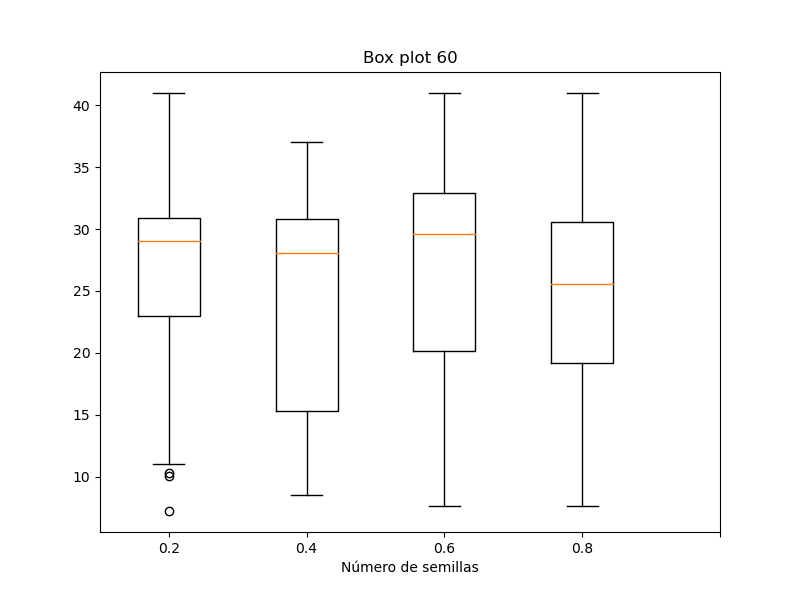
\includegraphics[width=\linewidth]{Fig60.png}
		\caption{Tamaño de la zona 60x60.}
		\label{60}
	\end{subfigure}
		\begin{subfigure}[b]{0.45\linewidth}
		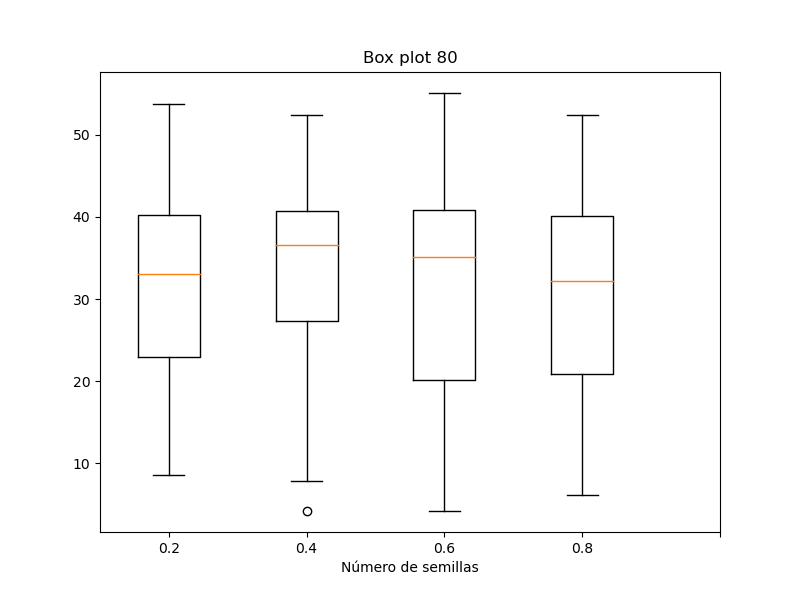
\includegraphics[width=\linewidth]{Fig80.png}
		\caption{Tamaño de la zona 80x80.}
		\label{80}
	\end{subfigure}
		\begin{subfigure}[b]{0.45\linewidth}
			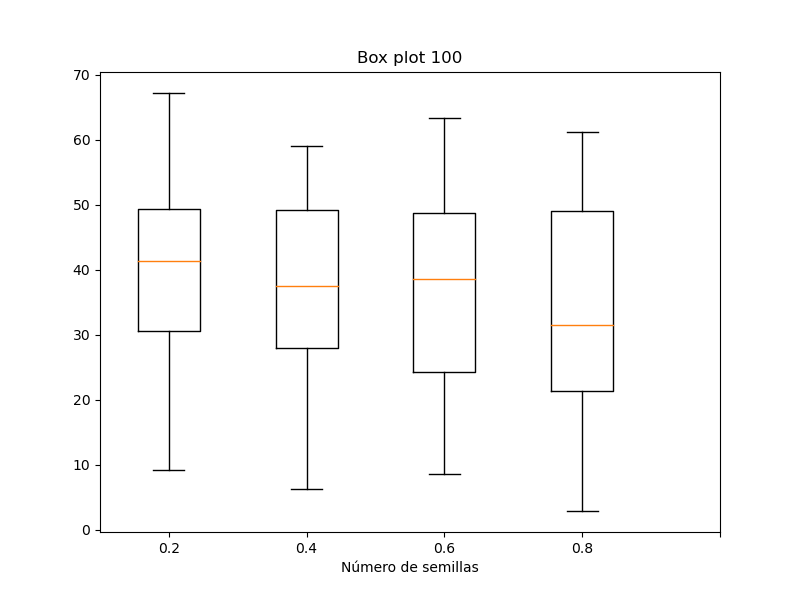
\includegraphics[width=\linewidth]{Fig100.png}
			\caption{Tamaño de la zona 100x100.}
			\label{100}
	\end{subfigure}
		\begin{subfigure}[b]{0.45\linewidth}
				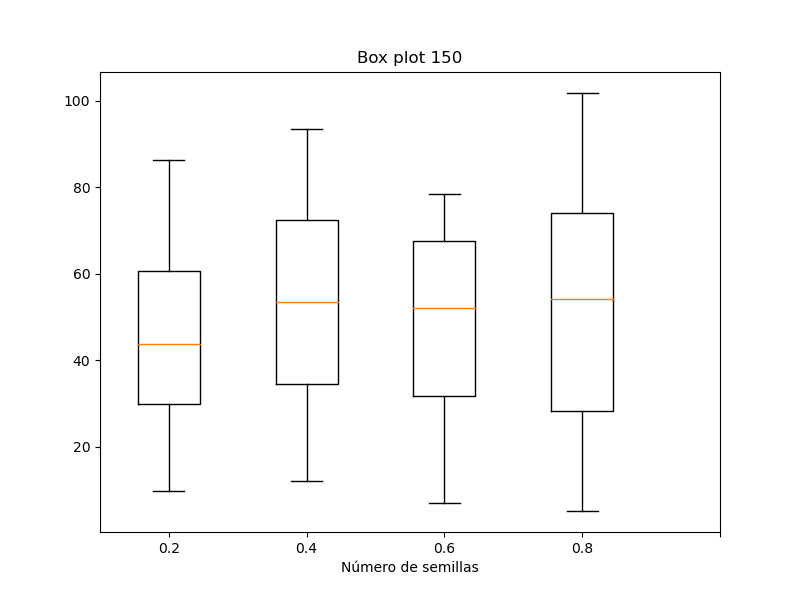
\includegraphics[width=\linewidth]{Fig150.png}
				\caption{Tamaño de la zona 150x150.}
				\label{150}
	\end{subfigure}
	\caption{Resultados por  tamaño de la zona y número de semillas.}  		
\end{figure}


Para el experimento de la figura 2 se sometió a una variación de la probabilidad inicial de propagación y se guardaron los datos para la zona más grande la de 150x150 y observar el comportamiento de dichos datos. Se muestra que no ocurre mucha variación en la distancia a la que llegan las grietas, sí cambia el comportamiento en cuanto a estabilidad.

\begin{figure}
	\centering
	\begin{subfigure}[b]{0.45\linewidth}
		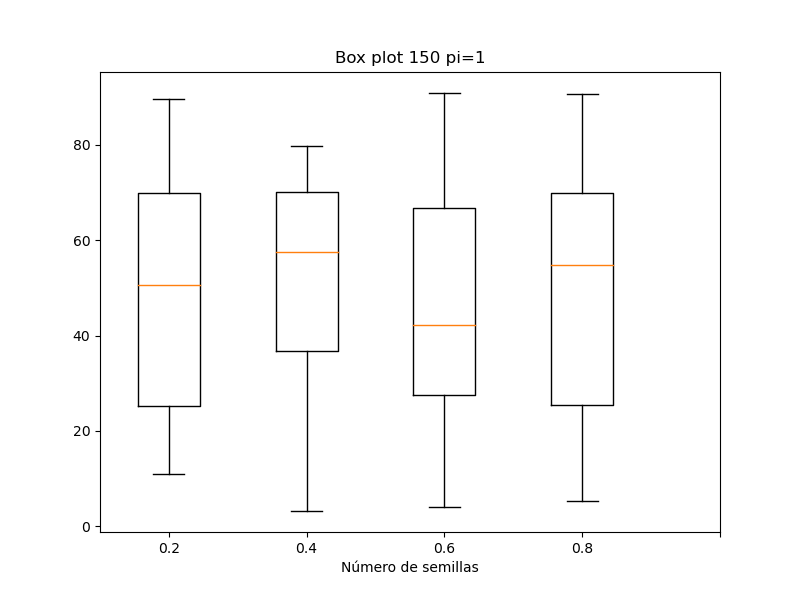
\includegraphics[width=\linewidth]{Figp1.png}
		\caption{Probabilidad inicial 0.9.}
		\label{09}
	\end{subfigure}
		\begin{subfigure}[b]{0.45\linewidth}
			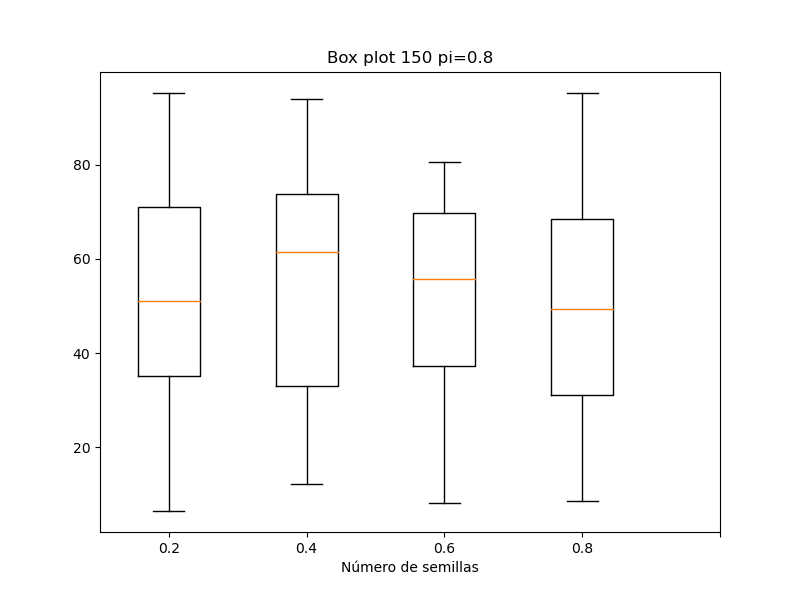
\includegraphics[width=\linewidth]{Figp8.png}
			\caption{Probabilidad inicial 0.8.}
			\label{08}
	\end{subfigure}
		\begin{subfigure}[b]{0.45\linewidth}
			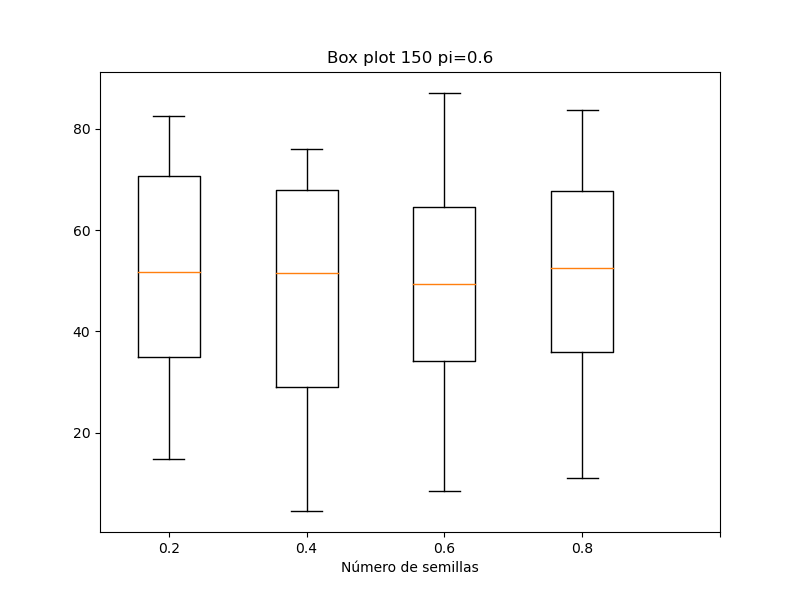
\includegraphics[width=\linewidth]{Figp6.png}
			\caption{Probabilidad inicial 0.6.}
			\label{06}
	\end{subfigure}
	\caption{Resultados para cambios de probabilidad de aparición de semillas en zona 150x150.}  		
\end{figure}

\section{Conclusiones}
Se puede concluir con los experimentos realizados que el aumento de las zonas para un mismo número de semillas, va a disminuir la distancia en la que se propaga la grieta, al hacer que las zonas centrales (las que se consideran más seguras) sean más grandes. En una misma zona si se le varía la probabilidad de aparición de semillas, se ve una disminución en la longitud de las grietas. Si se aumentan ambas, zonas y semillas existe un comportamiento más estable con respecto a la longitud de las grietas.

\bibliography{Tarea4}
\bibliographystyle{plainnat}
\end{document} 
